\input{include/perl-conf.tex}
\lstset{
%   texcl=true,
  keepspaces=true,
}

\newcommand{\slidefoot}[1]{
    \par\vspace{0.4em}{
        \footnotesize\color{black}#1
    }
}

\usepackage[normalem]{ulem} % \sout{} для зачёркивания

\title{Test2: жизнь после Test::More}
\author{Ликсанин Игорь}
\position{Backend разработчик,\\АО «Объединенные Цифровые Сети»}
\begin{document}
\titleframe

% Plan
\begin{frame}[fragile]{О чём расскажу}
    \begin{enumerate}
        \item TODO
    \end{enumerate}
\end{frame}

% Author frame
\authorframe{
  {\small
    \begin{itemize}
        \vspace{-\baselineskip} % убрать лишний зазор сверху
        \item 8 лет в Perl: 4 года full-stack,\\ 4 года только backend
        \item Перешёл в разработку из тестирования
        \item Контакты:\\
            \hspace*{1em}Telegram: \texttt{@iliksanin}\\
            \hspace*{1em}Email: \texttt{i.liksanin@mail.ru}
    \end{itemize}
  }
}

\begin{frame}[fragile]{Краткая история тестирования в Perl}
    \begin{itemize}
        \item Был изобретён TAP (\textit{Test Anything Protocol}).
        \item Разработчики вручную писали строки вывода, например: \texttt{print "ok - Test passed\textbackslash n";}.
        \item Появились подпрограммы для автоматизации: \texttt{ok()} и подобные.
        \item Стали появляться библиотеки объединиящие такие функции.
        \item Возникали проблемы из-за их несовместимости.
    \end{itemize}
\end{frame}

\begin{frame}[fragile]{Краткая история тестирования в Perl}
    \begin{itemize}
        \item Michael Schwern выпустил \texttt{Test::Builder} как совместимую основу, породив экосистему \texttt{Test::Builder}.
        \item Schwern и другие пытались переработать \texttt{Test::Builder} для исправления недостатков, но проект закрыли.
        \item Chad Granum выпустил \texttt{Test2} и обновил \texttt{Test::Builder}, превратив его в совместимый слой поверх \texttt{Test2}.
    \end{itemize}
\end{frame}

\begin{frame}[fragile]{Экосистема \texttt{Test::Builder}}
    \begin{itemize}
        \item \texttt{Test::Builder} - первая удачная попытка создать базу, на которой можно строить совместимые тестовые инструменты.
        \item \texttt{Test::Builder} привёл к бурному росту инструментов тестирования, которые надёжно работали вместе.
        \item Это была первая тестовая экосистема Perl.
    \end{itemize}
\end{frame}

\begin{frame}[fragile]{Экосистема \texttt{Test::Builder}}
    \begin{itemize}
        \item По мере её развития выявились изъяны и ограничения:
        \begin{itemize}
            \item Реализовать по-настоящему полезный \texttt{DieOnFail} почти невозможно.
            \item Проверка тестовых инструментов сводится к перехвату и валидации вывода \texttt{TAP}.
            \item Очень мало хуков для поведения, выходящего за рамки текстового вывода.
            \item \textit{Subtests} возможны и реализованы, но внутренности, делающие их рабочими, пугающе сложны и хрупки.
        \end{itemize}
    \end{itemize}
\end{frame}

\begin{frame}[fragile]{Test::More — заслуженный ветеран}
    \begin{itemize}\setlength\itemsep{1.2ex}
        \item Появился в 2001 году
        \item Стандарт де-факто для Perl-тестирования
        \vspace{0.25em}
        \begin{itemize}
            \setlength{\itemsep}{0.5ex}
            \item Входит в ядро Perl (с версии 5.6.2)
            \item Множество тестов написаны на нём
        \end{itemize}
        \item Простой и понятный API
        \vspace{0.25em}
        \begin{itemize}
            \setlength{\itemsep}{0.5ex}
            \item \texttt{ok(), is(), like(), done\_testing()}
            \item Легко освоить новичкам
        \end{itemize}
        \item Покрывает 80\% потребностей
        \vspace{0.25em}
        \begin{itemize}
            \setlength{\itemsep}{0.5ex}
            \item Базовые проверки
            \item Для сложных сценариев требуются дополнительные модули (\texttt{Test::Deep, Test::MockObject} и т.д.)
        \end{itemize}
    \end{itemize}
\end{frame}

\begin{frame}[fragile]{Проблемы Test::More: хрупкость}
    \begin{itemize}
        \item \texttt Test::More построен вокруг единого глобального объекта Test::Builder. Весь код тесно связан:\\
        \inputcode{Perl}{snippets/001.pl}\\
        Проблема: Невозможно изолировать части тестов или создать независимые тестовые контексты.
    \end{itemize}
\end{frame}

\begin{frame}[fragile]{Проблемы Test::More: хрупкость}
    \begin{itemize}
        \item Расширяющие функционал модули заменяли синглтон \texttt{Test::Builder}\\
        \inputcode{Perl}{snippets/002.pl}\\
    \end{itemize}
    Это одно из первых изменений которое зародило идею создания Test2
    \slidefoot{Подробнее: \url{https://perldoc.perl.org/Test2::Transition}}
\end{frame}

\begin{frame}[fragile]{Проблемы Test::More: хрупкость}
    \centering
    \hspace{0.5cm}
    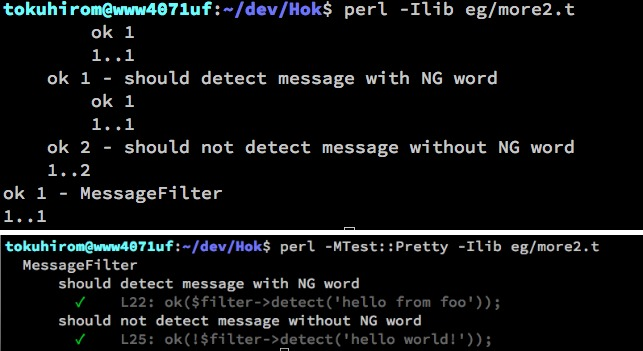
\includegraphics[height=\textheight]{snippets/format.jpg}
    \slidefoot{Подробнее: \url{https://github.com/tokuhirom/Test-Pretty/issues/25}}
\end{frame}

\begin{frame}[fragile]{Проблемы Test::More: хрупкость}
    \inputcode{Perl}{snippets/003.pl}
\end{frame}

\begin{frame}[fragile]{Проблемы Test::More:: хрупкость}
    \inputcode{Perl}{snippets/004.pl}
\end{frame}

\begin{frame}[fragile]{Проблемы Test::More: утечки памяти}
    \inputcode{Perl}{snippets/005.pl}
\end{frame}

\begin{frame}[fragile]{Неудобства Test::More: UTF8}
    \begin{itemize}
        \item При использовании utf8 с \texttt{Test::More} нужно не забывать сделать это с уважением\\
    \end{itemize}
    \inputcode{Perl}{snippets/006.pl}
\end{frame}

\begin{frame}[fragile]{Неудобства Test::More: прочие}
    \begin{itemize}
        \item Отсутствие встроенной поддержки моков
        \item Отсутствие встроенной поддержки тестов исключений и предупреждений
        \item Отсутвие встроенной поддержки гибкого глубокого сравнения
        \item Перемешивание в TAP строк детей при форках
        \item Рекомендации в документации по \texttt{Test::More} не использовать \texttt{Test::More} :)
    \end{itemize}
\end{frame}

\begin{frame}[fragile]{Test2 - революция или эволюция?}
    \begin{itemize}
        \item \textbf{Эволюция в использовании}
        \begin{itemize}
            \item Совместимость: \texttt{Test::Builder} теперь слой над \texttt{Test2}
            \item Привычные \texttt{ok/is/like/subtest} есть в \texttt{Test2::V0}
            \item Улучшения "из коробки": красивый \texttt{Compare} с таблицами, \texttt{Subtest} с буферизацией
        \end{itemize}

        \item \textbf{Революция в архитектуре}
        \begin{itemize}
            \item События вместо глобального состояния
            \item Плагины могут безопасно модифицировать поведение
            \item Легко создавать библиотеки не опасаясь сломать чужой код
        \end{itemize}
    \end{itemize}
\end{frame}

\begin{frame}[fragile]{Что такое \texttt{Test2}}
    \begin{itemize}
        \item \texttt{Test2} - это фреймворк для написания тестовых инструментов
        \item Упрощает написание собственных расширений
        \item Предоставляет множество инструментов из коробки \texttt{Test2::Suite}
    \end{itemize}
    \slidefoot{Подробнее: \url{https://perldoc.perl.org/Test2::Suite}}
\end{frame}


\begin{frame}[fragile]{А что будет с \texttt{Test::Builder}?}
    \begin{itemize}
        \item Сейчас \texttt{Test::Builder} - совместимый слой поверх \texttt{Test2}
        \item В таком виде с 10 мая 2016 года
        \item Можно смешивать инструменты из \texttt{Test::Builder} и \texttt{Test2}
        \item Вероятно он так и останется для совместимости со старым кодом
    \end{itemize}
\end{frame}

\begin{frame}[fragile]{\texttt{Test2::Suite}}
    \begin{itemize}
        \item Начиная с \texttt{Perl 5.40} \texttt{Test2::Suite} входит в core
        \item Вскоре \texttt{Test2::Suite} также будет объединён с дистрибутивом \texttt{Test-Simple}
        \item Уже сейчас можно использовать в модулях ядра (со слов автора \texttt{Test2})
    \end{itemize}

    \begin{columns}[c]
        \begin{column}{0.30\textwidth}
            \centering
            \includegraphics[width=0.85\linewidth]{snippets/TPRC-2024.png}
        \end{column}
        \begin{column}{0.70\textwidth}
            {\small Подробнее про экосистему Test2 от Chad Granum:}\\
            \url{https://www.youtube.com/watch?v=DdSQkIfeoqU}
        \end{column}
    \end{columns}
\end{frame}

\begin{frame}[fragile]{Test::More и Test2::V0}
    \only<1>{
        \inputcode{Perl}{snippets/007.pl}
        \vspace{0.5em}

        \begin{columns}[T,onlytextwidth]
            \begin{column}{0.49\textwidth}
            \lstinputlisting{snippets/007-1.txt}
            \end{column}
            \begin{column}{0.49\textwidth}
            \lstinputlisting{snippets/007-2.txt}
            \end{column}
        \end{columns}
    }
    \only<2>{
        \inputcode{Perl}{snippets/008.pl}
        \vspace{0.5em}

        \begin{columns}[T,onlytextwidth]
            \begin{column}{0.49\textwidth}
            \lstinputlisting{snippets/008-1.txt}
            \end{column}
            \begin{column}{0.49\textwidth}
            \lstinputlisting{snippets/008-2.txt}
            \end{column}
        \end{columns}
    }
    \only<3>{
        \inputcode{Perl}{snippets/009.pl}
        \vspace{0.5em}

        \begin{columns}[T,onlytextwidth]
            \begin{column}{0.49\textwidth}
            \lstinputlisting{snippets/009-1.txt}
            \end{column}
            \begin{column}{0.49\textwidth}
            \lstinputlisting{snippets/009-2.txt}
            \end{column}
        \end{columns}
    }
\end{frame}
\end{frame}


\begin{frame}[fragile]{TODO}
    \begin{enumerate}
        \item TODO
    \end{enumerate}
\end{frame}

\finalframe
\end{document}
